\chapter{基准环境实验}
在本章节,我们将会介绍测试HAAR算法和对比该算法与现有的最为先进算法的区别时,用到的实验环境。我们将会介绍强化学习社区在连续动作空间的任务上常用的基准实验环境,详述搭建方法和参数,以及汇报我们的实验结果。

\section{基准环境智能体介绍}
%强化学习社区统一的一套实验方案
强化学习社区经常采用的实验环境有Atari~\cite{atari_2013},Mujoco~\cite{benchmarking_RL}等等。其中,Mujoco仿真环境是连续动作空间的一个主要实验场景。我们的HAAR算法就致力于解决连续动作空间的问题,最终希望能够把它应用于机器人上。在这一节,我们将介绍Mujoco仿真环境。

Mujoco是一个物理仿真引擎。如图\ref{fig:mujoco}所示,(a)的名字为游泳体(Swimmer),游泳体由两个关节组成,通过在水中扭动身体达到前进的目的。(b)-(d)为一系列的二维运动体,比如猎豹、单足人、双足人,(e)为蚂蚁,由八个关节组成,与地面有一定的摩擦力,通过控制形态可以行走。(f)和(g)为两种人体建模,其中(f)的人体上半身具有较多的自由度。

	\begin{figure}[h] % use float package if you want it here
        \centering
        \includegraphics[scale=1.3]{mujoco/mujoco_models}
        \caption{(a)-(g)为强化学习社区常用的几个智能体。}
        \label{fig:mujoco}
    \end{figure}
    
强化学习算法通过在每一时刻计算这些智能体各关节需要施加的扭矩大小来控制智能体按照某种方式运动。也就是说,每一时刻的动作$a_t$为一个向量,其中每一维就表示各个关节对应的力矩。智能体对环境的观察$o_t$就表征了强化学习算法中的$s_t$,是可以自定义的。在上文提到的诸多智能体当中,我们主要采用蚂蚁和游泳体作为研究对象。这是因为,蚂蚁和游泳体的运动本身相对简单,并且可以扩展到二维空间的复杂地形中。

\section{实验环境搭建}
%介绍几个环境的共同点,特点,与之前的算法比有什么区别
在这一节我们设计了几个环境场景。这些场景设计的灵感来源是Mujoco基准环境提出者~\cite{benchmarking_RL}提出的``层次类问题''。所谓层次类问题,需要智能体进行高层和底层的决策。高层的决策类似于常见机器人问题(例如自动驾驶)中的``规划''问题,而底层的决策类似于常见机器人问题中的``控制''问题。基准环境~\cite{benchmarking_RL}一文中提出这样两类层次问题:``运动+食物收集''(Locomotion + Food Collection)和``运动+走迷宫''(Locomotion + Maze)问题。接下来,我们会对这两类问题都进行研究。

	\begin{figure}[h] % use float package if you want it here
        \centering
        \includegraphics[scale=0.35]{mujoco/env}
        \caption{(a) - (d)为我们设计的几个主要实验场景。(a)(b)是蚂蚁+迷宫,其中(b)环境是(a)环境的镜像,这在之后我们做迁移学习的时候会有用。(c)是游泳体+迷宫,(d)是蚂蚁+食物收集。(a)(b)(c)中红色箭头分别表示三者的目标位置。}
        \label{fig:exp_overview}
    \end{figure}

\subsection{观察空间设计}
注意到在这些实验当中,智能体对环境的观察是自定义的。因此,不同的强化学习算法在测试时往往会采用不同的环境观察。在以往的许多工作中,分层强化学习算法几乎都使用了智能体的$x, y$坐标作为观察的输入。有一些算法选择输入一个整体迷宫的俯视图,相当于变相告知智能体他所处的位置。这些处理方式大大简化了问题。因为,对于一个迷宫类的问题,其真正的难度在于智能体如何根据当前的局部环境来决定行动。也就是说,智能体需要拥有一定的``推测''能力。在第二章中我们对这个问题有过探讨。因此,我们在设计观察空间的时候,通过一定的安排使得底层策略是与具体任务和环境无关的,而上层策略是与单一任务无关,具备一定的泛化能力的。

具体来说,对于走迷宫问题,底层策略只知道智能体自身的关节角度和角速度,存储在$s^l$内,而上层策略只看到自身关节角度、角速度以及周围的局部环境状况,存储在$s^h$内。上层策略对于周围环境的感知取决于20条从智能体质心发出的``射线''。这些射线一旦接触到物体(如墙壁)便会记录这些接触点到智能体质心的距离$d_i$。射线最远能达到的距离定义为传感器量程$D$。记$s^h$当中对于周围环境信息的记录部分为$s^h_e$,我们定义
\begin{align}
  s^h_e = [\frac{d_i}{D}]^T
\end{align}

在这里我们采用``强度''(intensity)作为距离的表征而非距离本身,这是因为智能体离墙越近,受到的影响就应该越大,所以这样表示方便神经网络进行计算,是合理的。注意这里的物体可能是墙也可能是目标。为了在任何时刻都给智能体提供一定的参考,我们规定,即使目标被墙壁遮挡,我们也让它知道目标所在的位置。这一设定对于智能体来说简化了问题,是否会显著影响最终学习表现,我们在后文会进行横梁。

上述观察空间的设计使得我们的算法具备一定的泛化能力,可以在不同任务之间进行转移,我们在\ref{sec:transfer}节当中对此进行了讨论。

\vspace{0.5cm}
\textbf{蚂蚁迷宫环境}

蚂蚁迷宫环境如图\ref{fig:exp_overview}(a)和\ref{fig:ant_maze}所示。

\begin{figure}[h]
    \centering
    \includegraphics[width=0.9\textwidth]{mujoco/ant_maze}
    \caption{蚂蚁迷宫仿真环境中的一次训练。}
    \label{fig:ant_maze}
\end{figure}
图中,蚂蚁需要从起点出发,走到红色箭头所标注的目标位置。迷宫被划分为了$9 \times 9$的格子,蚂蚁只要进入目标所在位置的格子,我们就认为它成功完成此项任务。蚂蚁如果能够到达最终目标节点,我们就给它$1000$的奖励值,并且这一集会就此结束。如果在运动过程中摔倒,环境会给蚂蚁一个$-10$的奖励值,并且这一集经验会立刻结束。如果上述两种情况都没有发生,那么在第$1000$步,这一集经验也会自动终止。也就是说蚂蚁最多走1000步底层步。蚂蚁每次初始化的时候,都面向一个固定的方向。当迷宫发生镜像后,蚂蚁初始化姿态可能从面向出口改为面向墙壁。

\vspace{0.5cm}
\textbf{游泳体迷宫环境}

游泳体迷宫环境如图\ref{fig:exp_overview}(c)和\ref{fig:swimmer_maze}所示。

\begin{figure}[h]
    \centering
    \includegraphics[width=1.0\textwidth]{mujoco/swimmer_maze}
    \caption{游泳体迷宫仿真环境中的一场训练。}
    \label{fig:swimmer_maze}
\end{figure}
游泳体迷宫环境和蚂蚁类似。唯一的两个区别是,首先智能体从蚂蚁变成游泳体,在动力学方面更为简单;其次游泳体是不会摔倒的,所以它获得的唯一奖励是到达终点的1000奖励。游泳体每次出发的时候,都是横向起始的。游泳体迷宫问题其实是所有环境当中最简单的问题,因为游泳体比较稳定。但同时它的速度更慢,不灵活,因此探索过程会相对更为漫长。

\vspace{0.5cm}
\textbf{蚂蚁食物收集环境}

蚂蚁食物收集环境如图\ref{fig:exp_overview}(d)和\ref{fig:ant_gather}所示。

\begin{figure}[H]
    \centering
    \includegraphics[width=0.9\textwidth]{mujoco/ant_gather}
    \caption{蚂蚁食物收集仿真环境中的一场训练。左下角色条为蚂蚁对环境的观察。可以看到蚂蚁逐渐收集了绿色苹果并避开了红炸弹。}
    \label{fig:ant_gather}
\end{figure}
蚂蚁食物采集环境其实不是一个稀疏奖励问题。每次,在一个面积有限的环境中会随机产生一批食物和炸弹。如果蚂蚁走到食物,就会获得价值为1的奖励,如果蚂蚁走到炸弹,就会获得价值为-1的奖励,如果蚂蚁摔倒,就会获得价值为-10的奖励并且这一集经验采集结束。如果没有摔倒,蚂蚁会在走完1000小步以后自动结束。

\vspace{0.5cm}
\textbf{四房间环境}

为了增加实验难度,我们采用了一个蚂蚁四房间环境(图\ref{fig:ant_four_room})。这相当于难度更大的迷宫环境。我们特意破坏了四房间的对称性,这样就增大了环境的采样多样性。每次蚂蚁和目标都随机产生,蚂蚁走到目标获得价值为1000的奖励,摔倒为-10,蚂蚁能够走的最大步数为10,000步。
\begin{figure}[h]
    \centering
    \includegraphics[width=0.4\textwidth]{mujoco/four_room.png}
    \caption{蚂蚁四房间环境}
    \label{fig:ant_four_room}
\end{figure}

\subsection{随机起点}
前面提到了,在实际实验中,我们采取了``随机初始化''的采样方法。具体的,我们每一集经验采集的时候,会让蚂蚁从一个随机的位置初始化,每次终点位置固定。由于迷宫足够简单,因此我们认为这样已经可以随机化智能体的采样。对于复杂迷宫来说,需要我们对蚂蚁的起点和终点都进行随机化才能够让智能体在整个观察空间内随机采样。

采用随机起点法有两个初衷:首先,我们希望确保对不同状态空间采样的均匀性。加入一直让蚂蚁学习从最远端走到终点,那么一开始收集经验的时候,其实蚂蚁多数时候是不能走到终点的,这就导致采样数据一直停留在远离终点的位置附近,这会导致蚂蚁的策略对这局部的观察输入$s$非常敏感甚至过拟合。其次,我们希望上层策略学习到的知识是可迁移的,避免对特定点到点之间走法的过拟合。

随机起点法带来的一个附带好处是实际上降低了蚂蚁学习的难度。因为蚂蚁会有一定的几率离终点非常近,这样就可以在训练的初阶段获得一定的奖励值,从而先开始学习一些内容,逐渐把技能扩展到远处。但是这也导致我们的算法解决稀疏奖励问题的稀疏性较低,相当于变相地改变了解决的问题。并非所有的稀疏奖励问题都可以这样简化。因此在模型简化测试当中,我们也需要对是否随机化起点进行控制变量,观察是否有显著差异。

\section{实验结果及对比分析}
%视频实验结果截图;附上视频链接
我们把我们的算法HAAR和当前最为先进的分层强化学习算法作比较。其中,我们分别和SNN4HRL~\cite{SNN4hrl}算法,基于子目标的HAC ~\cite{HAC}和HIRO ~\cite{HIRO},以及非层次结构的TRPO~\cite{TRPO}算法在上述实验环境中进行比较。

注意到为了公平比较,HAAR和SNN4HRL算法共享了同样的下层初始策略,只不过SNN4HRL后续不会再更改这些初始化的底层策略。

实验结果表明,HAAR算法远远好于许多和我们对比的基线算法。图\ref{fig:learning_curve}当中展示了其中的一些对比结果。注意,所有的曲线都是经历5个不同的随机种子运行后,进行平均的结果。淡颜色的误差范围表示的是$95\%$的置信区间。在所有实验当中,我们都加进了一个不带有底层技能执行长度退火的实验结果来检验底层技能长度退火对于我们训练效果的影响。实验的详细参数和实施细节可以在第\ref{params}节当中找到。

我们的视频可以在这个网站链接\footnote{视频详见\url{http://bit.ly/2JxA0eN}}查看到。

\begin{figure}[ht]
    \centering
    \includegraphics[width=1.0\textwidth]{exp/learning_curve}
    \caption{成功率或者任务获得回报的学习曲线。分别对应了蚂蚁迷宫环境,游泳体迷宫环境,和蚂蚁收集食物环境。学习曲线分别是带有退火的HAAR(HAAR with skill annealing),不带有退火的HAAR(HAAR without skill length annealing),SNN4HRL以及TRPO。}
    \label{fig:learning_curve}
\end{figure}

\subsection{与SNN4HRL和非层次结构算法的对比}

和SNN4HRL相比, HAAR在图\ref{fig:exp_overview}的(a),(c)和(d)实验当中都取得了更快的学习速度和更好地学习结果。这证明了仅仅使用预训练的底层策略并不足以在需要层次化结构的问题中取得好的效果。

通过对底层策略的进一步优化,我们的算法能够让蚂蚁机器人稳定地行走,在切换底层技能的时候不会摔倒,也获得了更高的收敛值(成功率)。

SNN4HRL在游泳体迷宫环境中的成功率比在蚂蚁迷宫环境中更高。这是因为,即使底层策略不进一步优化,游泳体也不会在切换底层策略的过渡位置摔倒。尽管如此,HAAR算法在游泳体迷宫问题当中仍然取得了比SNN4HRL更好的结果。在图\ref{fig:learning_curve}(b)中可以看到,HAAR在不到200个迭代过后,就几乎达到了$100\%$的成功率。

对于蚂蚁收集环境来说,最大的挑战其实不在于稀疏奖励问题,而在于问题的复杂性。在蚂蚁收集环境当中,食物和炸弹都非常密集,因此环境的反馈并不稀疏。虽然HAAR是为稀疏奖励问题设计的,但是在蚂蚁收集环境中依然取得了比基线算法更好的结果。这说明HAAR也可以用于非稀疏奖励的问题当中,并仍然可以体现出其层次结构的优势。

TRPO是一个非层次结构的算法,并不能解决时间线长的稀疏奖励问题。TRPO在蚂蚁迷宫环境中和游泳体迷宫环境中的成功率都几乎为0。在蚂蚁收集环境中,蚂蚁能够收获一定的增长,因为它学会待在原地不动,由此不会摔倒获得$-10$的死亡奖励,也可以避免炸弹的负向奖励。

\subsection{与基于子目标的方法对比} 

我们也把HAAR与其他最前沿的,基于子目标方法的HRL算法进行了对比。包括HAC和HIRO算法,并在蚂蚁迷宫这一环境中进行了比较。由于我们使用了一个比较现实的观察空间表示,利用扫描传感器,不包含智能体的$x, y$坐标信息,这些基于子目标的HRL算法不能够很好地计算当前状态与子目标状态的距离,因此和非层次结构的强化学习算法TRPO表现一样。我们甚至还通过把目标直接放在蚂蚁面前的方法来简化这个任务,但是这些算法依然难以学会让蚂蚁向前走。因此,我们没有在实验结果中保留这些算法的学习曲线。

这个结果与我们先前关于基于子目标的HRL算法的分析相同。这也在2018年的一篇文章~\cite{sensitive_to_goal_space}中被进行了仔细的分析。这篇文章对状态空间的表示进行了一些变异,但没有我们从$x, y$变成扫描传感器的变化这么剧烈,而这些算法依然只取得了很差的表现。

\subsection{可视化技能和轨迹}
\label{deeper}

为了展示HAAR算法是如何获得和其他算法相比更优的表现的,我们在本节中提供了一种对底层技能和整体任务轨迹可视化的方法。我们将分别对蚂蚁迷宫和游泳体迷宫的轨迹进行分析。

\begin{figure*}[htbp]
\centering
 \centering
    \includegraphics[width=0.9\textwidth]{exp/ant_skill}
\caption{(a) 蚂蚁预训练底层技能的访问历史图。 (b) 蚂蚁在蚂蚁迷宫环境中训练过后的底层技能访问历史图。 (c) 训练过后,蚂蚁在蚂蚁迷宫环境中的两条示例轨迹。}
\label{fig:ant_detail}
\end{figure*}

在图\ref{fig:ant_detail}当中, (a) 和 (b) 分别展示了在训练之前和训练之后,一系列的底层技能访问历史图。在这些图中,蚂蚁总是从中间$(0, 0)$位置出发,不断采用同一个底层策略,走500步走出的轨迹。对比(b)和(a),我们可以发现蚂蚁学会了右转策略(黄色的技能1)和直走(红色的技能0)并且在迷宫任务 (c)当中很好地使用了这两个策略。在(c)中,蚂蚁试图从S走到G。我们可以清晰地看到蚂蚁切换技能的过程。

和蚂蚁迷宫问题相似,游泳体迷宫问题也显示出经过HAAR的训练后,智能体对下层策略的一定改变是有意义的。
在图 \ref{fig:swimmer_skill}(a)(b)中,游泳体每次都在中间的$(0, 0)$位置初始化,并且初始身体状态是水平的。每次游泳体都执行同一个底层技能若干步,多次执行后得到了这样的访问历史图。 (c)展示了若干条游泳体从其实节点S走到目标节点G的轨迹曲线。我们可以看到,游泳体学会了修改它的底层策略,从而实现了更加有效率的移动能力。

\begin{figure}[htbp]
    \centering
    \includegraphics[width=0.9\textwidth]{exp/swimmer_skill.pdf}
    \caption{游泳体底层技能的展示。(a) 游泳体在HAAR训练之前的底层技能访问历史图。 (b) 游泳体在HAAR训练之后的底层技能访问历史图。 (c) 游泳体在迷宫中游动路径的展示。 }
    \label{fig:swimmer_skill}
\end{figure}

在我们的算法框架中,我们不对智能体底层策略的初始化方式作任何的假设。我们的主要贡献在于,设计了一个辅助奖励函数用于促进底层策略的训练。

\subsection{四房间问题}

\begin{wrapfigure}{r}{6cm}
\includegraphics[width=0.4\textwidth]{exp/four_room}
\setlength{\belowcaptionskip}{-1.0cm}
\caption{四房间问题当中,HAAR算法和SNN4HRL算法的对比,没有显著差异。}
\label{fig:four_room_learning_curve}
\end{wrapfigure}

我们单独在这一节分析四房间问题。四房间问题的环境构建如图\ref{fig:ant_four_room}所示。四房间问题比其他的问题更为复杂,也因此需要更多地采样和算力。通过实验我们发现,如图\ref{fig:four_room_learning_curve}展示的那样,HAAR并没有比单纯的SNN获得更好的结果,但这两者都远远好于非层次结构的TRPO算法。这与之前的实验有显著的差异。我们认为,HAAR表现不好的原因可能是(1)参数没有仔细设计(2)采样不够充足(3)限于算力,我们只进行了50个迭代,进行更多步的迭代后增长曲线在后期可能会出现显著区别(4)四房间问题本身的复杂性导致HAAR算法也不能解决,而随机初始化位置带来的一些简单情形HAAR和SNN4HRL相比并没有优势。具体是哪个原因,还有待进一步的实验研究。

\subsection{状态空间表示和迁移学习}\label{sec:transfer}
我们在实验中发现了一个有趣的现象。尽管HAAR最初并不是为迁移学习设计的,在实验中,$\pi_h$和$\pi_l$都能够迁移到相似的任务当中去。在这一节,我们将介绍这个迁移的现象,并分析HAAR算法可迁移性背后可能的原因。

HAAR算法对于状态空间的具体表示方法是没有要求的。因此,在实验中我们进行了一个基于现实机器人传感器能力的限定,希望让我们的智能体只能接触到在所有任务中都统一具备的一些信息。首先,像我们在之前定义的那样,$s^l$ 是智能体的``自我观察值''。这保证了底层策略是不清楚自身周围情况的,因此限定于基本的元动作,例如向前走,但是不会依据环境发生改变。这能够防止层次结构退化为单层结构——假如底层策略也能够访问周围环境的信息,这个技能可能进化为在整个迷宫中都能使用,而上层策略每次都只选择这个下层技能~\cite{feudal}~\cite{option-critic}。

\begin{wrapfigure}{r}{6cm}
\includegraphics[width=0.45\textwidth]{exp/transferred}
\setlength{\belowcaptionskip}{0.0cm}
\caption{在蚂蚁地图环境\ref{fig:exp_overview}(b)中,迁移来自(a)习得的策略。分别是迁移上下层策略,只迁移下层策略,和完全不迁移(即原版HAAR)的学习曲线。}
\label{fig:transfer}
\end{wrapfigure}

上层策略除了在$s^l$有的信息以外,还可以通过一个扫描传感器去访问周围的物体。我们禁止智能体获得自身绝对坐标,因此他不会简单地记住自己一直在训练的这个环境,而会学会归纳总结。在图\ref{fig:transfer}当中展示的实验证明了HAAR的上层和下层策略都具备可迁移性。

在这个迁移性实验中,我们从之前图\ref{fig:ant_maze}(a)的训练结果中随机挑选一个$\pi_l$和它对应的上层策略$\pi_h$,并直接在图\ref{fig:ant_maze}(b)环境当中跑。图\ref{fig:transfer}展示了同时迁移$\pi_h$和$\pi_l$的时候,成功率在一开始就有一个$0.2$的起跳。同时,可以看出这个方法的学习速度也远远快于不迁移的方法。只迁移底层策略$\pi_l$也能够加快训练速度,但是并没有同时迁移上下层的效果那么明显。这证明了$\pi_l$和$\pi_h$都是可迁移的,并且在新任务学习当中起到了积极地作用。相比之下,像HIRO~\cite{HIRO}一类观察值依赖于绝对坐标的算法,是不可能同时迁移上下层策略的(因为上层策略取决于坐标,而换个环境坐标系就会发生显著改变)。

我们想要指出的是,在这个实验中我们仅仅使用了一个简单的迷宫。这个智能体在此迷宫中训练,对于环境观察值多多少少还是有一些过拟合。假如我们使用更为复杂的迷宫,就应该能够解决这个过拟合问题。


\section{模型简化测试:控制变量}
在这一节里,我们想要探索一些问题。我们的方法采用了很多细节处理,这些细节处理是否都对智能体的学习有用?为了解决这个问题,我们采用控制变量的方法研究这些细节发生改变时,是否会带来不同的训练结果。我们希望探究以下问题:
\begin{enumerate}
  \item 底层技能长度退火算法对训练速度是否有影响?
  \item 随机起点法对训练速度和结果是否有影响?
  \item 用同时训练近似交替训练是否会影响优化的单调性?
  \item 实验中,被墙遮挡的目标对智能体是否可见是否会影响训练?
  \item 采用HAAR方法和直接使用环境奖励在训练结果上是否有显著差异?
  \item 辅助奖励和其他环境反馈(如蚂蚁的摔倒奖励值)相比,哪个对底层技能优化的影响更大?
\end{enumerate}

\subsection{底层技能长度退火算法对训练的影响}
不使用底层技能长度退火的HAAR算法和使用底层技能退火的HAAR在训练的最后都拥有同样的底层技能长度。这样就可以保证两者在训练结束的时候获得了结构上相同的策略。在此基础上,我们比较两种训练方法对训练的影响。

图\ref{fig:learning_curve}的(a)(b)(c)当中都展示了两种方法的学习曲线。大体上来说,底层技能长度退火的训练方法能够帮助智能体更快地学习。并且退火这个行为本身并不会对最终的结果有任何显著的影响。 这是因为,最终的结果不论在训练过程中有没有采用退火,都会用到同样的底层技能长度$k$。我们在算法部分对这个结果也进行过详细的讨论,其基本思路在于,当$k$比较大时,上层策略面临的问题更为简单,因为他只需要通过较少的步数就可以走到终点。技能长度退火相当于一种课程学习的思想(curriculum learning),为上层策略逐渐增加任务难度。$k$比较小的时候,技能会比较灵活,能够更快地对状态的改变作出反应,因此整体策略也容易更优。

\subsection{采用随机起点法对训练的影响}
注意到在实验部分,我们采用了随机起点的方法。我们提到这种方法能够降低任务难度。但是,随机起点法是否在HAAR完成任务的过程中起到了决定性作用呢?为了研究HAAR是否能够独立于随机起点方法存在,从而能解决更一般的稀疏奖励问题,我们需要进行三个不同的对比试验:(1)不随机产生起点(2)等概率随机产生起点(3)我们实际采用的方法:为了保证采样的均匀性,我们应该以更高的概率在越远离终点的地方产生起点(因为远离终点的地方要达到目标总要经过离终点更近的地方,反之不然)。

通过初步的实验,我们发现随机起点的具体方法不会对成功率产生显著的影响。

\subsection{同时训练和交替训练的区别}
\label{appendix:concurrent}

\begin{figure}[!ht]
    \centering
    \includegraphics[width=0.5\textwidth]{concurrent_VS_alternate}
    \caption{对比同时优化和交替优化得到的结果。}
    \label{fig:concurrent}
\end{figure}

回忆我们在HAAR算法证明的开始提出了一个重要的假设。我们认为,HAAR对于上下层策略的单调递增性可以保证,要求我们在优化$\pi_l$的时候$\pi_h$是固定的,而我们优化$\pi_h$的时候$\pi_h$是固定的。这个假设成立当且仅当,我们采集一批经验以后,我们要么依据这批经验优化$\pi_h$,要么只优化$\pi_l$而不能同时优化两者。这样做的一个例子就是,不断采集经验,利用每批经验每次交替地优化$\pi_h$和$\pi_l$。

但是在实际操作的时候,HAAR每采集一批经验,就同时优化了$\pi_h$和$\pi_l$。为了研究这样做是否会破坏HAAR的单调优化性能,我们对比了这样操作的学习曲线和严格的,交替训练上下层的方法。我们在蚂蚁迷宫这一环境中使用两种方法进行训练。

如图 \ref{fig:concurrent}所示,同时优化上下层策略(蓝色曲线)带来的训练速度是交替优化上下层策略(橙色曲线)的两倍,而并没有改变成功率的收敛值。这就说明,每次不严格地同时训练上下层得到的训练结果并不会比每次只训练上层或下层要差。同时,这样做还能大大提高采样效率,减少训练耗时。因此,我们利用实验说明了HAAR算法是安全的。

\subsection{能否观察到被遮挡的目标对于训练的影响}
接下来我们将介绍为了完整验证结论,未来需要完善的一些实验内容。首先,我们在实验中有这样一个设计,简化了任务的难度:当智能体离目标很远时,即使目标被墙遮挡,我们也让它能够看到目标。这样设计的思路在于,当智能体完全接收不到目标信息时,它的探索是无任何信息含量的,而人类在走迷宫的时候往往预先知道目标的存在,因此即使人类没有走到目标,其探索也是有信息含量的。实际中,当目标被遮挡时,这个问题就变成了一个部分可观测的马尔科夫决策问题(POMDP)。我们想探索HAAR算法能否在这个更具挑战性的环境里完成任务。

\subsection{HAAR和直接采用环境反馈训练区别的显著性}
由于优势函数也是上层基于环境的反馈学习出来的,一个自然的问题是,我们的方法是否真的能够解决环境所不能解决的问题?为了研究这个问题,我们进行了额外的实验,把环境的反馈直接返回给智能体的下层策略。实验结果表明,利用环境奖励直接反馈给下层,会导致智能体学习速度非常缓慢,仅比完全不训练下层略快一点。这说明HAAR设计的辅助奖励是有效的,效果远好于直接使用环境奖励本身。

\subsection{其他奖励值和辅助奖励函数对于训练的贡献}
注意到在涉及到蚂蚁的环境中,我们对预先训练好的下层进行进一步训练的时候,不仅提供了辅助奖励函数,还提供了一个摔倒的反馈。为了衡量最终究竟是我们设计的奖励函数起到主要作用还是摔倒的反馈起到了主要作用,我们需要控制变量。

在游泳体迷宫的实验中,我们已经训练了智能体从起点走到终点。由于游泳体除了最终到达目标获得的奖励以外再无别的奖励输入(如摔倒),这个实验结果可以部分地证明辅助奖励的确是对训练起到了作用。

进一步的实验需要我们对比这些不同的奖励(辅助奖励、摔倒奖励)对训练结果作用的影响大小。这要求我们在蚂蚁迷宫的环境中补充实验。我们将进行这样的实验设计:一个实验为只给蚂蚁摔倒奖励,不给辅助奖励;另一个实验为既给蚂蚁摔倒奖励,也给蚂蚁辅助奖励(即HAAR实际采用的算法)。只有当第二个实验的学习曲线上升速度超过第一个实验,才能充分证明我们算法的有效性。

\section{实验参数和细节}\label{params}
\subsection{超参数}
现将在实验中可能会影响到HAAR算法表现的超参数列举如下。首先我们需要确定利用SNN4HRL~\cite{SNN4hrl}预训练底层策略的迭代次数$N$,这决定了底层策略的好坏。 我们还需要确定每次采集一批经验的时候,限定一共采集多少步的底层步数$B$,上下层策略分别有自己的折扣率$\gamma_h$和$\gamma_l$,每一集经验中最大底层步数$T$,每一个上层步骤下底层步骤数量$k_s$(在不退火的情况下)和初始步长$k_0$(在采取退火的情况下)。注意到我们总是这样定义退火温度:在这个温度下,我们让智能体在训练进行到一半的时候恰好步长收敛到最终步长$k_s$。(大约在$\frac{B}{2}$的地方)我们没有对这些参数进行详细的区间搜索,而是直接根据经验和建议指定,因此我们的算法在一定条件下可能可以得到更好的结果。这也侧面印证了HAAR算法的鲁棒性。

我们利用了rllab~\cite{benchmarking_RL}当中定义好的蚂蚁智能体。上层状态$s^h$ 的观察包含了蚂蚁的``自我观察''(关节的角度和角速度),并且也能够通过扫描传感器的20条射线观察到周围的墙壁和目标。底层策略则只能看到蚂蚁的自身观察量。

表\ref{table:hyperparamters}当中展现了在各个实验平台都需要设定的参数。

\begin{table}
\caption{统一超参数列表}
\begin{tabular}[c]{ |p{3cm}||p{3cm}|p{3cm}|p{3cm}|  }
 \hline 
 \multicolumn{4}{|c|}{Hyperparameters for experiments} \\
 \hline
 Hyperparameter & Ant Maze & Swimmer Maze & Ant Gather \\
 \hline
 N  & $1000$ & $500$ & $3000$\\
 B  & $5\times 10^4$ & $5\times10^5$  & $5\times10^4$ \\
 $\gamma_l$ & $0.99$ & $0.99$ & $0.99$\\
 $\gamma_h$ & $0.99$ & $0.99$ & $0.99$\\
 $k_0$ & $100$  & $1000$ & $100$\\
 $k_s$ & $10$  & $500$  & $10$\\
 $T$ & $1000$  & $5000$ & $1000$\\
 \hline
\end{tabular}
\label{table:hyperparamters}
\end{table}

接下来,我们介绍几个具体实验环境中各自单独用到的一些参数。

\textbf{蚂蚁迷宫环境}

我们利用一系列$4\times4$的块状物体构建了一个``C''形的迷宫。这些块状物体要么是实心墙块,要么是空地。每一集经验结束,当且仅当蚂蚁到达目标(并获得价值$1000$的奖励),摔倒(并获得价值为$-10$的奖励),或者花费了最大时间长度。蚂蚁的目标放在一个$4\times4$的格子内,只要蚂蚁的质心进入这个格子,我们就认为蚂蚁成功到达目标。

\textbf{游泳体迷宫环境}

游泳体迷宫环境和蚂蚁迷宫环境采用了相同的迷宫。每一集经验结束,当且仅当游泳体到达目标或者是用光了所有时间($1000$步)。游泳体不会摔倒。

\textbf{蚂蚁食物收集环境}

蚂蚁在一个$6\times6$的地图环境去采集食物。一共随机产生了8个食物和8个炸弹。如果蚂蚁走到了食物的地方,它就会获得一个价值为$1$的奖励。一旦蚂蚁触碰到一次炸弹,就会获得价值为$-1$的惩罚。摔倒奖励值为$-10$。

\subsection{训练细节}
最后我们介绍一下训练神经网络当中的细节。

对于 $\pi_h$和$\pi_l$,我们都采用了简单的两层感知机网络,其中有32个隐藏单元。
对于驾驶函数$V(s)$,我们采用一个简单的多项式拟合,也就是$V(s) = W_3s^3 + W_2s^2 + W_1s + W_0$,注意这里的$s$其实是向量,$s^2$表示该向量的每一位都取平方。TRPO的优化步长为0.01。

对于预训练底层策略,我们没有改变SNN4HRL原文的设定,也就是规定有6个底层策略。蚂蚁在HAAR训练时,每一集经验走的最大底层步数为$50,000$,游泳体是$500$。超参数$\alpha_H$被设为$1$,这是SNN4HRL预训练时的超参数,其含义是共同信息熵的系数(MI bonus)。

\section{本章小结}
在本章中,我们通过大量仿真环境的实验,验证了HAAR算法的优越性。特别地,我们进行了许多控制变量的分析,剖析了HAAR算法中各个环节的作用和重要性,从而验证辅助函数的设计这一根本思想的有效性。为了方便复现,我们详细说明了实验的设计以及参数。在Mujoco仿真环境中,HAAR算法都取得了比以往算法更为优越的结果。
